\documentclass[a4paper, 12pt]{article}

\usepackage[T1]{fontenc}
\usepackage[left=3cm, right=3cm, top=4cm, bottom=4cm]{geometry}
\usepackage{amssymb}
\usepackage{amsmath}
\usepackage{booktabs}
\usepackage{setspace}
\usepackage{float}
\usepackage{mathtools}
\usepackage{makecell}
\usepackage{longtable}
\usepackage{caption}
\usepackage{graphicx}

\captionsetup[longtable]{skip=8pt}

\newcommand{\code}[1]{\texttt{#1}}

\newcommand{\R}{\mathbb{R}}

\DeclarePairedDelimiter\abs{\lvert}{\rvert}

\onehalfspacing

\title{
  Obliczenia Naukowe\\
  \begin{center}\Large Lista 2\end{center}
}
\author{Piotr Kocia}

\begin{document}

\maketitle

\tableofcontents

\section{Problem 1}
Calculate the inner product of two vectors $\tilde{x}$ and $y$, and compare with $\left< x, y \right>$
\begin{gather*}
  x = [2.718281828, -3.141592654, 1.414213562, 0.5772156649, 0.3010299957] \\
  \tilde{x} = [2.718281828, -3.141592654, 1.414213562, 0.577215664, 0.301029995] \\
  y = [1486.2497, 878366.9879, -22.37492, 4773714.647, 0.000185049]
\end{gather*}
using 4 different methods: naive, reverse naive, sorted partial sums in
descending order, sorted partial sums in ascending order.

\subsection{Solution}
The code may be found in \code{ex1.jl}. Generic functions are used to reduce
code duplication.

\subsection{Results}
\begin{table}[H]
\centering
\begin{tabular}{@{}rcccc@{}}
\toprule
                   & Float32 $x$             & Float32 $\tilde{x}$   \\ \midrule
Naive Forward      & -0.4999443              & -0.4999443            \\ \midrule
Naive Backward     & -0.4543457              & -0.4543457            \\ \midrule
Partial Descending & -0.5                    & -0.5                  \\ \midrule
Partial Ascending  & -0.5                    & -0.5                  \\ \bottomrule
\end{tabular}
\caption{Comparison of the results of the different inner product methods in the
Float32 arithmetic.}
\label{tab:inner_products_f32}
\end{table}

\begin{table}[H]
\centering
\begin{tabular}{@{}rcccc@{}}
\toprule
                   & Float64 $x$             & Float64 $\tilde{x}$   \\ \midrule
Naive Forward      & 1.0251881368296672e-10  & -0.004296342739891585 \\ \midrule
Naive Backward     & -1.5643308870494366e-10 & -0.004296342998713953 \\ \midrule
Partial Descending & 0.0                     & -0.004296342842280865 \\ \midrule
Partial Ascending  & 0.0                     & -0.004296342842280865 \\ \bottomrule
\end{tabular}
\caption{Comparison of the results of the different inner product methods in the
Float64 arithmetic.}
\label{tab:inner_products_f64}
\end{table}

\subsection{Conclusions}
The exact result is $-1.00657107000000 \cdot 10^{-11}$ and as may be seen the
results in Table \ref{tab:inner_products_f32} and Table
\ref{tab:inner_products_f64} differ greatly. While the introduction of a minor
corruption of data in the Float32 arithmetic does not alter the results (the
precision is too low), the Float64 arithmetic suffers greatly. We may conclude
that such great error is caused by the problem being ill-conditioned.

\section{Problem 2}
Graph the function $f(x) = e^x \ln\left(1+e^{-x}\right)$ and compare to the
limit of the function.

\subsection{Solution and Results}
We graph function $f$ in two graphing calculators - desmos (Figure \ref{fig:desmos}) and WolframAlpha (Figure \ref{fig:wolfram}).

\begin{figure}
\centering
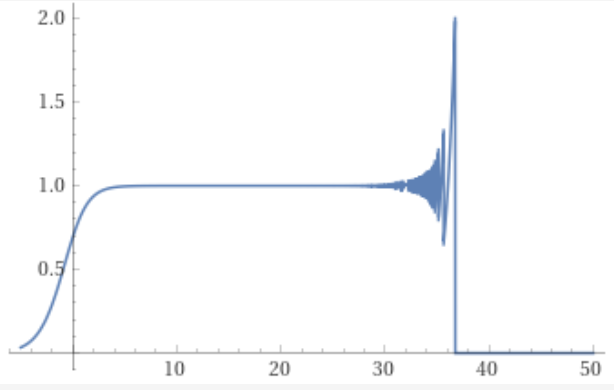
\includegraphics[width=0.75\linewidth]{wolfram.png}
\caption{$f(x)$ plotted in WolframAlpha.}
\label{fig:wolfram}
\end{figure}
\begin{figure}
\centering
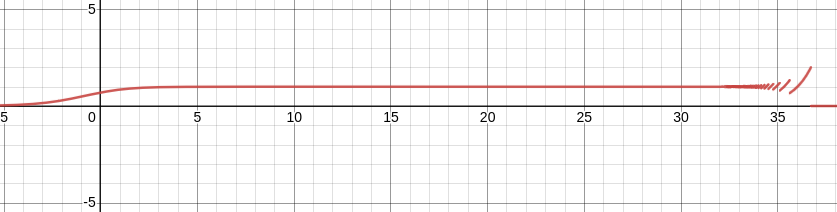
\includegraphics[width=0.75\linewidth]{desmos.png}
\caption{$f(x)$ plotted in desmos.}
\label{fig:desmos}
\end{figure}

We now calculate the limit of $f$
\begin{align*}
\lim_{x \to \inf} f(x) &= \lim_{x \to \inf} e^x\ln\left(1+e^{-x}\right) \\
&\stackrel{\text{L'Hopital}}{=} \lim_{x \to \inf} \frac{-1}{e^x + 1} \frac{1}{-e^{-x}} \\
&= \lim_{x \to \inf} \frac{e^x}{e^x + 1} \\
&= \lim_{x \to \inf} \frac{e^x + 1 - 1}{e^x + 1} \\
&= \lim_{x \to \inf} \left(1 - \frac{1}{e^x + 1}\right) \\
&= 1
\end{align*}

\subsection{Conclusions}
The graphs of $f$ appear correct until around $x = 30$ when the precision of the
underlaying arithmetic becomes insufficient and fails. The problem stems from
the fact that $e^x$ is a rapidly increasing exponential, similarly $e^{-x}$ is a
rapidly decreasing function. In the term $\ln(1 + e^{-x})$ the value inside the
logarithm approaches 1, the whole term tends to 0 quickly and, due to
insufficient precision, becomes 0, which may be observed in both Figure
\ref{fig:desmos} and Figure \ref{fig:wolfram}.

\section{Problem 3}
Using two methods of solving linear equations:
\begin{itemize}
\item Gaussian elimination,
\item left mutliplication by the inverse matrix,
\end{itemize}
for a given matrix $A \in \R^{n \times n}$ and a given column vector $b \in
\R^{n}$, solve
\begin{equation}
Ax = b
\end{equation}
and calculate the relative error $\abs{\frac{x - \tilde{x}}{x}}$, where $x$ is
the exact solution and $\tilde{x}$ is the calculated solution.

For the matrix $A$ we will be substituting:
\begin{itemize}
\item the Hilbert matrix $H_n$,
\item a matrix $C = R^n$ with the condition number $c$,
\end{itemize}
and for $x$ a column vector of 1s. From there we will calculate $b$ and then
solve for $x$.

\subsection{Solution}
The solution may be found in \code{ex3.jl}. All calculations are done in Float64
arithmetic.

\subsection{Results}
\begin{table}[H]
\centering
\begin{tabular}{@{}cccc@{}}
\toprule
n  & Condition Number      & Gauss Error            & Inverse Error          \\ \midrule
1  & 1.0                   & 0.0                    & 0.0                    \\ \midrule
2  & 19.28147006790397     & 5.661048867003676e-16  & 1.4043333874306803e-15 \\ \midrule
3  & 524.0567775860644     & 8.022593772267726e-15  & 0.0                    \\ \midrule
4  & 15513.73873892924     & 4.137409622430382e-14  & 0.0                    \\ \midrule
5  & 476607.2502425855     & 1.6828426299227195e-12 & 3.3544360584359632e-12 \\ \midrule
6  & 1.4951058642254734e7  & 2.618913302311624e-10  & 2.0163759404347654e-10 \\ \midrule
7  & 4.753673567446793e8   & 1.2606867224171548e-8  & 4.713280397232037e-9   \\ \midrule
8  & 1.5257575538060041e10 & 6.124089555723088e-8   & 3.07748390309622e-7    \\ \midrule
9  & 4.9315375594102344e11 & 3.8751634185032475e-6  & 4.541268303176643e-6   \\ \midrule
10 & 1.602441698742836e13  & 8.67039023709691e-5    & 0.0002501493411824886  \\ \midrule
11 & 5.222701316549833e14  & 0.00015827808158590435 & 0.007618304284315809   \\ \midrule
12 & 1.7515952300879806e16 & 0.13396208372085344    & 0.258994120804705      \\ \midrule
13 & 3.1883950689209334e18 & 0.11039701117868264    & 5.331275639426837      \\ \midrule
14 & 6.200786281355982e17  & 1.4554087127659643     & 8.71499275104814       \\ \midrule
15 & 3.67568286586649e17   & 4.696668350857427      & 7.344641453111494      \\ \midrule
16 & 7.046389953630175e17  & 54.15518954564602      & 29.84884207073541      \\ \midrule
17 & 1.249010044779401e18  & 13.707236683836307     & 10.516942378369349     \\ \midrule
18 & 2.2477642911280653e18 & 10.257619124632317     & 24.762070989128866     \\ \midrule
19 & 6.472700911391398e18  & 102.15983486270827     & 109.94550732878284     \\ \midrule
20 & 1.1484020388436145e18 & 108.31777346206205     & 114.34403152557572     \\ \bottomrule
\end{tabular}
\caption{The relative error of the solution of the equation with the hilbert matrix $H^n$.}
\label{tab:error_hilbert}
\end{table}

\begin{table}[H]
\centering
\begin{tabular}{@{}cccc@{}}
\toprule
n  & Condition Number      & Gauss Error            & Inverse Error          \\ \midrule
5  & 1.0000000000000004    & 2.0471501066083611e-16 & 1.4043333874306804e-16 \\ \midrule
5  & 10.000000000000018    & 2.808666774861361e-16  & 1.7901808365247238e-16 \\ \midrule
5  & 1000.0000000000616    & 1.590775652421124e-14  & 1.7165067669544676e-14 \\ \midrule
5  & 9.999999990176475e6   & 2.4656888773357746e-11 & 7.809377196826238e-11  \\ \midrule
5  & 1.0000108585997009e12 & 4.9932111484190324e-5  & 4.292170159617677e-5   \\ \midrule
5  & 9.527049327005712e15  & 0.21189462094396352    & 0.20799451615367168    \\ \midrule
10 & 1.0000000000000013    & 2.830524433501838e-16  & 2.673771110915334e-16  \\ \midrule
10 & 10.000000000000007    & 1.7901808365247238e-16 & 3.475547814546182e-16  \\ \midrule
10 & 1000.000000000056     & 4.5386264868992765e-15 & 5.803822934319861e-15  \\ \midrule
10 & 9.99999999585611e6    & 2.7702052655817713e-11 & 2.3839454895894454e-11 \\ \midrule
10 & 9.999981309580488e11  & 1.2232240466804122e-5  & 1.1385641738503112e-5  \\ \midrule
10 & 8.301575543479199e15  & 0.05805461029170589    & 0.06717160058969304    \\ \midrule
20 & 1.0000000000000009    & 3.657001166779273e-16  & 4.839349969133126e-16  \\ \midrule
20 & 10.000000000000005    & 4.523392502223303e-16  & 5.376277206893598e-16  \\ \midrule
20 & 999.9999999999274     & 1.5915696643323185e-14 & 1.567861342173416e-14  \\ \midrule
20 & 9.99999999724386e6    & 5.09221779309765e-11   & 9.074551467751946e-11  \\ \midrule
20 & 9.999773851442334e11  & 9.592928534698156e-6   & 7.66803967579849e-6    \\ \midrule
20 & 9.518203800017898e15  & 0.09378984366663241    & 0.11401968374473768    \\ \bottomrule
\end{tabular}
\caption{The relative error of the solution of the equation with the condition matrix $C$.}
\label{tab:error_condition}
\end{table}

\subsection{Conclusions}
In the Hilbert matrix case it is clearly visible that the problem is
ill-conditioned - the condition number explodes and the error quickly exceeds 1
and goes into hundreds meaning our results are about as good as random guesses.

On the other hand, the relative error of the solutions with the $C$ matrix
depends on the condition number of the matrix as varying the size seems to have
little effect.

We may also conclude that if a matrix has a high condition number, the problem
of solving the equation $Ax = b$ becomes ill-condition regardless of the matrix
used.

\section{Problem 4}
The Wilkinson polynomial is given by
\begin{align*}
P(x) = \ &x^{20} - 210x^{19} + 20615x^{18} - 1256850x^{17} + 53327946x^{16}
\tag{explicit form}\\
&- 1672280820x^{15} + 40171771630x^{14} - 756111184500x^{13} \\
&+ 11310276995381x^{12} - 135585182899530x^{11} +1307535010540395x^{10} \\
&- 10142299865511450x^{9} + 63030812099294896x^{8} - 311333643161390640x^{7} \\
&+ 1206647803780373360x^{6} - 3599979517947607200x^{5} \\
&+ 8037811822645051776x^{4} - 12870931245150988800x^{3} \\
&+ 13803759753640704000x^{2} - 8752948036761600000x \\
&+ 2432902008176640000 \\
p(x) = \ &(x - 20)(x - 19)(x - 18)(x - 17)(x - 16) \tag{factor form} \\
& (x - 15)(x - 14)(x - 13)(x - 12)(x - 11) \\
& (x - 10)(x - 9)(x - 8)(x - 7)(x - 6) \\
& (x - 5)(x - 4)(x - 3)(x - 2)(x - 1)
\end{align*}
Calculate the roots $z_k$ from the explicit from and evaluate both forms at
$z_k$. Additionally, apply a perturbation to the polynomial by subtracting
$2^{-23}$ from the coefficient $a_19$ and explain the differences.

\subsection{Solution}
The solution may be found in \code{ex4.jl}.

\subsection{Results}

\begin{table}[H]
\centering
\begin{tabular}{@{}cccc@{}}
\toprule
$k$ & $z_k$              & $\abs{P(z_k)}$        & $\abs{p(z_k)}$ \\ \midrule
1   & 0.9999999999996989 & 35696.50964788257     & 5.518479490350445e6 \\ \midrule
2   & 2.0000000000283182 & 176252.60026668405    & 7.37869762990174e19 \\ \midrule
3   & 2.9999999995920965 & 279157.6968824087     & 3.3204139316875795e20 \\ \midrule
4   & 3.9999999837375317 & 3.0271092988991085e6  & 8.854437035384718e20 \\ \midrule
5   & 5.000000665769791  & 2.2917473756567076e7  & 1.8446752056545688e21 \\ \midrule
6   & 5.999989245824773  & 1.2902417284205095e8  & 3.320394888870117e21 \\ \midrule
7   & 7.000102002793008  & 4.805112754602064e8   & 5.423593016891273e21 \\ \midrule
8   & 7.999355829607762  & 1.6379520218961136e9  & 8.262050140110275e21 \\ \midrule
9   & 9.002915294362053  & 4.877071372550003e9   & 1.196559421646277e22 \\ \midrule
10  & 9.990413042481725  & 1.3638638195458128e10 & 1.655260133520688e22 \\ \midrule
11  & 11.025022932909318 & 3.585631295130865e10  & 2.24783329792479e22 \\ \midrule
12  & 11.953283253846857 & 7.533332360358197e10  & 2.886944688412679e22 \\ \midrule
13  & 13.07431403244734  & 1.9605988124330817e11 & 3.807325552826988e22 \\ \midrule
14  & 13.914755591802127 & 3.5751347823104315e11 & 4.612719853150334e22 \\ \midrule
15  & 15.075493799699476 & 8.21627123645597e11   & 5.901011420218566e22 \\ \midrule
16  & 15.946286716607972 & 1.5514978880494067e12 & 7.010874106897764e22 \\ \midrule
17  & 17.025427146237412 & 3.694735918486229e12  & 8.568905825736165e22 \\ \midrule
18  & 17.99092135271648  & 7.650109016515867e12  & 1.0144799361044434e23 \\ \midrule
19  & 19.00190981829944  & 1.1435273749721195e13 & 1.1990376202371257e23 \\ \midrule
20  & 19.999809291236637 & 2.7924106393680727e13 & 1.4019117414318134e23 \\ \bottomrule
\end{tabular}
\caption{The calculated roots of the Wilkinson polynomial and the value of the polynomial at them.}
\label{tab:wilk_roots}
\end{table}

\begin{table}[H]
\centering
\begin{tabular}{@{}cc@{}}
\toprule
$k$ & $\abs{z_k - k}$ \\ \midrule
1   & 3.0109248427834245e-13 \\ \midrule
2   & 2.8318236644508943e-11 \\ \midrule
3   & 4.0790348876384996e-10 \\ \midrule
4   & 1.626246826091915e-8 \\ \midrule
5   & 6.657697912970661e-7 \\ \midrule
6   & 1.0754175226779239e-5 \\ \midrule
7   & 0.00010200279300764947 \\ \midrule
8   & 0.0006441703922384079 \\ \midrule
9   & 0.002915294362052734 \\ \midrule
10  & 0.009586957518274986 \\ \midrule
11  & 0.025022932909317674 \\ \midrule
12  & 0.04671674615314281 \\ \midrule
13  & 0.07431403244734014 \\ \midrule
14  & 0.08524440819787316 \\ \midrule
15  & 0.07549379969947623 \\ \midrule
16  & 0.05371328339202819 \\ \midrule
17  & 0.025427146237412046 \\ \midrule
18  & 0.009078647283519814 \\ \midrule
19  & 0.0019098182994383706 \\ \midrule
20  & 0.00019070876336257925 \\ \bottomrule
\end{tabular}
\caption{The difference between the calculated roots and the exact roots.}
\label{tab:wilk_root_diff}
\end{table}

\begin{table}[H]
\centering
\begin{tabular}{@{}cc@{}}
\toprule
$z_k$              & $\tilde{z_k}$ \\ midrule
0.9999999999996989 & 0.9999999999998357 + 0.0im \\ \midrule
2.0000000000283182 & 2.0000000000550373 + 0.0im \\ \midrule
2.9999999995920965 & 2.99999999660342 + 0.0im \\ \midrule
3.9999999837375317 & 4.000000089724362 + 0.0im \\ \midrule
5.000000665769791  & 4.99999857388791 + 0.0im \\ \midrule
5.999989245824773  & 6.000020476673031 + 0.0im \\ \midrule
7.000102002793008  & 6.99960207042242 + 0.0im \\ \midrule
7.999355829607762  & 8.007772029099446 + 0.0im \\ \midrule
9.002915294362053  & 8.915816367932559 + 0.0im \\ \midrule
9.990413042481725  & 10.095455630535774 - 0.6449328236240688im \\ \midrule
11.025022932909318 & 10.095455630535774 + 0.6449328236240688im \\ \midrule
11.953283253846857 & 11.793890586174369 - 1.6524771364075785im \\ \midrule
13.07431403244734  & 11.793890586174369 + 1.6524771364075785im \\ \midrule
13.914755591802127 & 13.992406684487216 - 2.5188244257108443im \\ \midrule
15.075493799699476 & 13.992406684487216 + 2.5188244257108443im \\ \midrule
15.946286716607972 & 16.73074487979267 - 2.812624896721978im \\ \midrule
17.025427146237412 & 16.73074487979267 + 2.812624896721978im \\ \midrule
17.99092135271648  & 19.5024423688181 - 1.940331978642903im \\ \midrule
19.00190981829944  & 19.5024423688181 + 1.940331978642903im \\ \midrule
19.999809291236637 & 20.84691021519479 + 0.0im \\ \bottomrule
\end{tabular}
\caption{The roots of the Wilkinson polynomial and the roots of the modified polynomial.}
\label{tab:wilk_modified}
\end{table}

\subsection{Conclusions}
The Wilkinson polynomial is a prominent example of the fact that finding the
roots of a polynomial is in general an ill-conditioned problem. Even a small
perturbation ($2^-23$ in this case) results in a significant change of the
roots, therefore it is undesirable to naively use a root finding algorithm as an
intermediate step of a larger procedure because doing so might introduce extreme
ill-conditioning regardless of how well conditioned the original problem was.

The calculated roots are close to the exact values, but the error is
significant. Another problem present in this example is that we are severely
limited by the precision of the Float64 arithmetic, which leads to further
accumulation of error.

\section{Problem 5}
Given
\begin{equation}
p_{n+1} = p_n + rp_n(1-p_n), \mathrm{for} \ n = 0, 1, ...
\end{equation}
compute $p_n$ for $n = 0, 1, ... 40$ in Float32, Float64 and in Float32
truncating the result after 10 iterations to 3 significant digits.

\subsection{Solution}
The solution may be found in \code{ex5.jl}.

\subsection{Results}
\begin{table}[H]
\centering
\begin{tabular}{@{}ccc|ccc@{}}
\toprule
$n$ & Truncated   & Correct     & $n$ & Truncated   & Correct \\ \midrule
0   & 0.01        & 0.01        & 21  & 0.09289217  & 1.3107498 \\ \midrule
1   & 0.0397      & 0.0397      & 22  & 0.34568182  & 0.088804245 \\ \midrule
2   & 0.15407173  & 0.15407173  & 23  & 1.0242395   & 0.3315584 \\ \midrule
3   & 0.5450726   & 0.5450726   & 24  & 0.94975823  & 0.9964407 \\ \midrule
4   & 1.2889781   & 1.2889781   & 25  & 1.0929108   & 1.0070806 \\ \midrule
5   & 0.1715188   & 0.1715188   & 26  & 0.7882812   & 0.9856885 \\ \midrule
6   & 0.5978191   & 0.5978191   & 27  & 1.2889631   & 1.0280086 \\ \midrule
7   & 1.3191134   & 1.3191134   & 28  & 0.17157483  & 0.9416294 \\ \midrule
8   & 0.056273222 & 0.056273222 & 29  & 0.59798557  & 1.1065198 \\ \midrule
9   & 0.21559286  & 0.21559286  & 30  & 1.3191822   & 0.7529209 \\ \midrule
10  & 0.7229306   & 0.7229306   & 31  & 0.05600393  & 1.3110139 \\ \midrule
11  & 1.3241479   & 1.3238364   & 32  & 0.21460639  & 0.0877831 \\ \midrule
12  & 0.036488414 & 0.037716985 & 33  & 0.7202578   & 0.3280148 \\ \midrule
13  & 0.14195944  & 0.14660022  & 34  & 1.3247173   & 0.9892781 \\ \midrule
14  & 0.50738037  & 0.521926    & 35  & 0.034241438 & 1.021099 \\ \midrule
15  & 1.2572169   & 1.2704837   & 36  & 0.13344833  & 0.95646656 \\ \midrule
16  & 0.28708452  & 0.2395482   & 37  & 0.48036796  & 1.0813814 \\ \midrule
17  & 0.9010855   & 0.7860428   & 38  & 1.2292118   & 0.81736827 \\ \midrule
18  & 1.1684768   & 1.2905813   & 39  & 0.3839622   & 1.2652004 \\ \midrule
19  & 0.577893    & 0.16552472  & 40  & 1.093568    & 0.25860548 \\ \midrule
20  & 1.3096911   & 0.5799036 \\ \bottomrule
\end{tabular}
\caption{Comparison of truncated vs non-truncated iterations.}
\label{tab:model_truncated}
\end{table}

\begin{longtable}[H]{ccc}
\toprule
$n$ & Float32     & Float64              \\ \midrule \endhead
0   & 0.01        & 0.01                 \\ \midrule
1   & 0.0397      & 0.0397               \\ \midrule
2   & 0.15407173  & 0.15407173000000002  \\ \midrule
3   & 0.5450726   & 0.5450726260444213   \\ \midrule
4   & 1.2889781   & 1.2889780011888006   \\ \midrule
5   & 0.1715188   & 0.17151914210917552  \\ \midrule
6   & 0.5978191   & 0.5978201201070994   \\ \midrule
7   & 1.3191134   & 1.3191137924137974   \\ \midrule
8   & 0.056273222 & 0.056271577646256565 \\ \midrule
9   & 0.21559286  & 0.21558683923263022  \\ \midrule
10  & 0.7229306   & 0.722914301179573    \\ \midrule
11  & 1.3238364   & 1.3238419441684408   \\ \midrule
12  & 0.037716985 & 0.03769529725473175  \\ \midrule
13  & 0.14660022  & 0.14651838271355924  \\ \midrule
14  & 0.521926    & 0.521670621435246    \\ \midrule
15  & 1.2704837   & 1.2702617739350768   \\ \midrule
16  & 0.2395482   & 0.24035217277824272  \\ \midrule
17  & 0.7860428   & 0.7881011902353041   \\ \midrule
18  & 1.2905813   & 1.2890943027903075   \\ \midrule
19  & 0.16552472  & 0.17108484670194324  \\ \midrule
20  & 0.5799036   & 0.5965293124946907   \\ \midrule
21  & 1.3107498   & 1.3185755879825978   \\ \midrule
22  & 0.088804245 & 0.058377608259430724 \\ \midrule
23  & 0.3315584   & 0.22328659759944824  \\ \midrule
24  & 0.9964407   & 0.7435756763951792   \\ \midrule
25  & 1.0070806   & 1.315588346001072    \\ \midrule
26  & 0.9856885   & 0.07003529560277899  \\ \midrule
27  & 1.0280086   & 0.26542635452061003  \\ \midrule
28  & 0.9416294   & 0.8503519690601384   \\ \midrule
29  & 1.1065198   & 1.2321124623871897   \\ \midrule
30  & 0.7529209   & 0.37414648963928676  \\ \midrule
31  & 1.3110139   & 1.0766291714289444   \\ \midrule
32  & 0.0877831   & 0.8291255674004515   \\ \midrule
33  & 0.3280148   & 1.2541546500504441   \\ \midrule
34  & 0.9892781   & 0.29790694147232066  \\ \midrule
35  & 1.021099    & 0.9253821285571046   \\ \midrule
36  & 0.95646656  & 1.1325322626697856   \\ \midrule
37  & 1.0813814   & 0.6822410727153098   \\ \midrule
38  & 0.81736827  & 1.3326056469620293   \\ \midrule
39  & 1.2652004   & 0.0029091569028512065\\ \midrule
40  & 0.25860548  & 0.011611238029748606 \\ \bottomrule
\caption{Comparison of $p_n$ in Float32 and Float64.} \\
\label{tab:model_compare} \\
\end{longtable}

\subsection{Conclusions}
The results presented in Table \ref{tab:model_truncated} and Table
\ref{tab:model_compare} show that the precision used in calculating the next
values of $p_n$ is insufficient. The rounding error accumulates rapidly as $p_n$
is given by a recursive formula containing a square term effectively requiring
doubling of precision each iteration.

\section{Problem 6}
Given
\begin{equation}
x_{n+1} = x^2_n + c
\end{equation}
compute $x_n$ for $n = 1, 2, ..., 40$.

\subsection{Solution}
The solution may be found in \code{ex6.jl}.

\subsection{Results}
\begin{longtable}[H]{cccc}
\toprule
$n$ & $x_0 = 1.0$ & $x_0 = 2.0$ & $x_0 = 1.99...$ \\ \midrule \endhead
1  & -1.0 & 2.0 & 1.99999999999996     \\ \midrule
2  & -1.0 & 2.0 & 1.9999999999998401   \\ \midrule
3  & -1.0 & 2.0 & 1.9999999999993605   \\ \midrule
4  & -1.0 & 2.0 & 1.999999999997442    \\ \midrule
5  & -1.0 & 2.0 & 1.9999999999897682   \\ \midrule
6  & -1.0 & 2.0 & 1.9999999999590727   \\ \midrule
7  & -1.0 & 2.0 & 1.999999999836291    \\ \midrule
8  & -1.0 & 2.0 & 1.9999999993451638   \\ \midrule
9  & -1.0 & 2.0 & 1.9999999973806553   \\ \midrule
10 & -1.0 & 2.0 & 1.999999989522621    \\ \midrule
11 & -1.0 & 2.0 & 1.9999999580904841   \\ \midrule
12 & -1.0 & 2.0 & 1.9999998323619383   \\ \midrule
13 & -1.0 & 2.0 & 1.9999993294477814   \\ \midrule
14 & -1.0 & 2.0 & 1.9999973177915749   \\ \midrule
15 & -1.0 & 2.0 & 1.9999892711734937   \\ \midrule
16 & -1.0 & 2.0 & 1.9999570848090826   \\ \midrule
17 & -1.0 & 2.0 & 1.999828341078044    \\ \midrule
18 & -1.0 & 2.0 & 1.9993133937789613   \\ \midrule
19 & -1.0 & 2.0 & 1.9972540465439481   \\ \midrule
20 & -1.0 & 2.0 & 1.9890237264361752   \\ \midrule
21 & -1.0 & 2.0 & 1.9562153843260486   \\ \midrule
22 & -1.0 & 2.0 & 1.82677862987391     \\ \midrule
23 & -1.0 & 2.0 & 1.3371201625639997   \\ \midrule
24 & -1.0 & 2.0 & -0.21210967086482313 \\ \midrule
25 & -1.0 & 2.0 & -1.9550094875256163  \\ \midrule
26 & -1.0 & 2.0 & 1.822062096315173    \\ \midrule
27 & -1.0 & 2.0 & 1.319910282828443    \\ \midrule
28 & -1.0 & 2.0 & -0.2578368452837396  \\ \midrule
29 & -1.0 & 2.0 & -1.9335201612141288  \\ \midrule
30 & -1.0 & 2.0 & 1.7385002138215109   \\ \midrule
31 & -1.0 & 2.0 & 1.0223829934574389   \\ \midrule
32 & -1.0 & 2.0 & -0.9547330146890065  \\ \midrule
33 & -1.0 & 2.0 & -1.0884848706628412  \\ \midrule
34 & -1.0 & 2.0 & -0.8152006863380978  \\ \midrule
35 & -1.0 & 2.0 & -1.3354478409938944  \\ \midrule
36 & -1.0 & 2.0 & -0.21657906398474625 \\ \midrule
37 & -1.0 & 2.0 & -1.953093509043491   \\ \midrule
38 & -1.0 & 2.0 & 1.8145742550678174   \\ \midrule
39 & -1.0 & 2.0 & 1.2926797271549244   \\ \midrule
40 & -1.0 & 2.0 & -0.3289791230026702  \\ \bottomrule
\caption{Results for $c = -2$.} \\
\label{tab:recursive_c2} \\
\end{longtable}

\begin{longtable}[H]{ccccccc}
\toprule
$x_0 = 1.0$ & $x_0 = -1.0$ & $x_0 = 0.75$ & $x_0 = 0.2$ \\ \midrule \endhead
0.0  & 0.0  & -0.4375 & -0.96 \\ \midrule
-1.0 & -1.0 & -0.80859375 & -0.07840000000000003 \\ \midrule
0.0  & 0.0  & -0.3461761474609375 & -0.99385344 \\ \midrule
-1.0 & -1.0 & -0.8801620749291033 & -0.012255339800166465 \\ \midrule
0.0  & 0.0  & -0.2253147218564956 & -0.9998498066463825 \\ \midrule
-1.0 & -1.0 & -0.9492332761147301 & -0.00030036414919165644 \\ \midrule
0.0  & 0.0  & -0.0989561875164966 & -0.9999999097813779 \\ \midrule
-1.0 & -1.0 & -0.9902076729521999 & -1.804372361524642e-7 \\ \midrule
0.0  & 0.0  & -0.01948876442658909 & -0.9999999999999675 \\ \midrule
-1.0 & -1.0 & -0.999620188061125 & -6.505906924303417e-14 \\ \midrule
0.0  & 0.0  & -0.0007594796206411569 & -1.0 \\ \midrule
-1.0 & -1.0 & -0.9999994231907058 & 0.0 \\ \midrule
0.0  & 0.0  & -1.1536182557003727e-6 & -1.0 \\ \midrule
-1.0 & -1.0 & -0.9999999999986692 & 0.0 \\ \midrule
0.0  & 0.0  & -2.6616486792363503e-12 & -1.0 \\ \midrule
-1.0 & -1.0 & -1.0 & 0.0 \\ \midrule
0.0  & 0.0  & 0.0 & -1.0 \\ \midrule
-1.0 & -1.0 & -1.0 & 0.0 \\ \midrule
0.0  & 0.0  & 0.0 & -1.0 \\ \midrule
-1.0 & -1.0 & -1.0 & 0.0 \\ \midrule
0.0  & 0.0  & 0.0 & -1.0 \\ \midrule
-1.0 & -1.0 & -1.0 & 0.0 \\ \midrule
0.0  & 0.0  & 0.0 & -1.0 \\ \midrule
-1.0 & -1.0 & -1.0 & 0.0 \\ \midrule
0.0  & 0.0  & 0.0 & -1.0 \\ \midrule
-1.0 & -1.0 & -1.0 & 0.0 \\ \midrule
0.0  & 0.0  & 0.0 & -1.0 \\ \midrule
-1.0 & -1.0 & -1.0 & 0.0 \\ \midrule
0.0  & 0.0  & 0.0 & -1.0 \\ \midrule
-1.0 & -1.0 & -1.0 & 0.0 \\ \midrule
0.0  & 0.0  & 0.0 & -1.0 \\ \midrule
-1.0 & -1.0 & -1.0 & 0.0 \\ \midrule
0.0  & 0.0  & 0.0 & -1.0 \\ \midrule
-1.0 & -1.0 & -1.0 & 0.0 \\ \midrule
0.0  & 0.0  & 0.0 & -1.0 \\ \midrule
-1.0 & -1.0 & -1.0 & 0.0 \\ \midrule
0.0  & 0.0  & 0.0 & -1.0 \\ \midrule
-1.0 & -1.0 & -1.0 & 0.0 \\ \midrule
0.0  & 0.0  & 0.0 & -1.0 \\ \midrule
-1.0 & -1.0 & -1.0 & 0.0 \\ \bottomrule
\caption{Results for $c = -1$.} \\
\label{tab:recursive_c1} \\
\end{longtable}

\subsection{Conclusions}
For all $c$ and $x_0$ except $x_0 = 1.99999999999999$ the value of $x_n$
converges to a certain number (-1, 2) or oscillates between two numbers (0, -1).
The pair $x_0 = 1.99999999999999$, $c = -2$, however, does not converge within
40 iterations. This implies that the formula is sensitive to the initial
conditions.

\end{document}
